\documentclass[../proofs.tex]{subfiles}

\begin{document}
\chapter{Indirect Proofs}
% Indirect Proofs
An indirect proof method is a method in which the proof does not explicitly prove the desired predicate \footnote{A \emph{predicate} is a formal statement in mathematics that can either be seen as a true statement or a false statement. Predicates are what this note might informally refer to as `statements'}. An indirect proof resorts to proving another statement, for whose validity it immediately follows (or in other words, implies) the desired predicate's validity. We provide a classic example. \footnote{This is known as Euclid's Argument of infinite primes.} \\

% Euclid's Argument
\begin{expl}{Prove that there are infinitely many prime numbers.}
\begin{proof}
  Let $p$ be a prime number. Then $p$ satisfies the following conditions:
    \begin{enumerate}
      \item $p \in \mathbb{N}$
      \item $p \geq 2$, and
      \item The only factors of $p$ are $1$ and $p$, that is, no number other than $1$ and $p$ divides $p$ evenly.
    \end{enumerate}
  Suppose to the contrary that there exists a finite number $n$ of prime numbers. \\
  Then,we may, theoretically, gather the entire collection of these primes. Let us exhaustively describe this collection as $F = \{p_1, p_2, ..., p_n\}$ \footnote{This is known as a set, and the way we have described it is called an \emph{exhaustive} description of a set.}. \\
  Let the number $p'$ be the \emph{product of all of the primes in $F$}. We must have:
  \begin{align*}
    p' = p_1 \cdot p_2 \cdot ... \cdot p_n
  \end{align*}
  We see that $p'$ is definitely divisible by all of the primes in existence in $F$ (by supposition). \\
  Consider the number $p''  = p' + 1$. Notice that this number is not divisible by any of the primes in existence - to see this, notice that by dividing $p'' $ by any $p \in F$, we always will get a remainder of 1\footnote{Rigorously, we would consult a mathematical construct known as the \emph{division algorithm} - however, I believe the preceding argument intuitively suffices.}.\\

  It becomes clear that the only factors of $p''$ are 1, and $p''$ itself. We have effectively generated a \emph{new} prime number that was not in $F$, our supposed `complete' set of all prime numbers. We have reached a contradiction, and we could not have possibly constructed a finite collection of prime numbers in the first place. The desired result follows.
  \end{proof}
\end{expl}
The `indirect' portion of this proof is in the supposition statement. We suppose that the statement we are trying to prove is false, and by flawless logical reduction from this negation, we reach a contradiction. We then argue that the only flaw in our logic was the supposition itself, therefore, the actual desired conclusion must be true. Thus, by resorting to proving another related statement, the desired statement is proven\footnote{Notice that the `equivalent' statement that we have proven can be stated as: ``It is not the case that the set of prime numbers is finite".}. (This specific indirect proof technique is known as a \emph{Proof by Contradiction.})

% a simple diagram of proof structure
\begin{figure}[h]
\centering
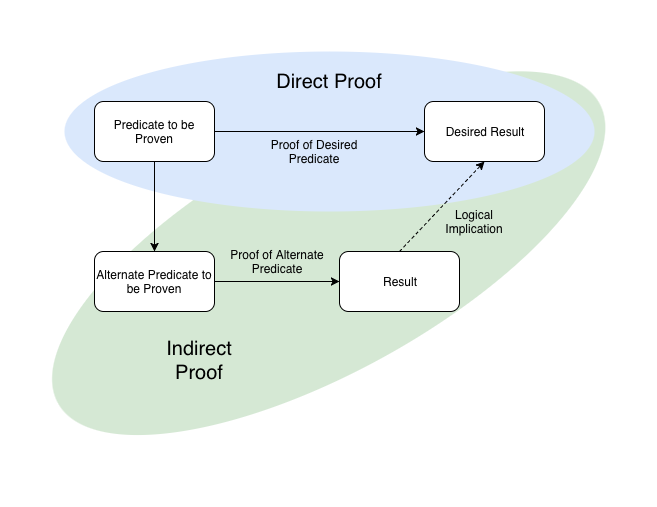
\includegraphics[scale=0.45]{res/direct_indirect.png}
\caption{The algorithmic difference between the two types of proof structure.}
\end{figure}
\end{document}
